% Created by tikzDevice version 0.12.3.1 on 2022-02-12 21:50:36
% !TEX encoding = UTF-8 Unicode
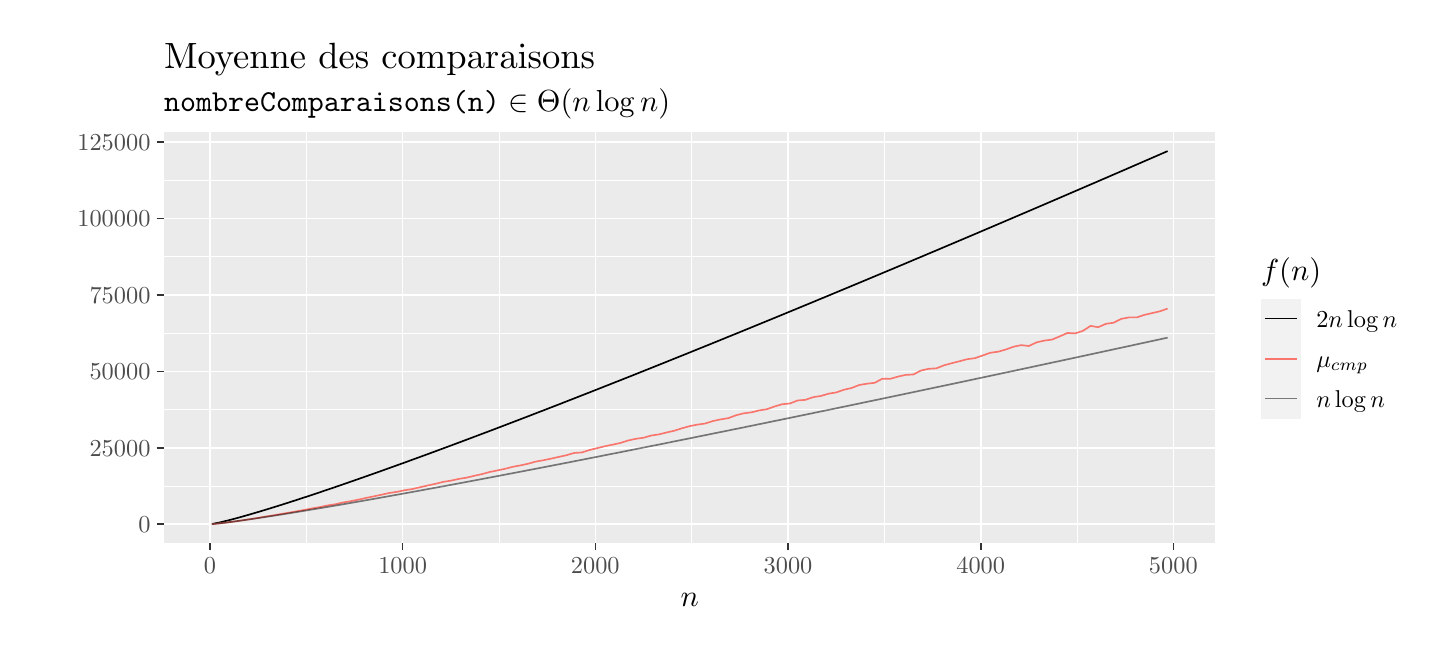
\begin{tikzpicture}[x=1pt,y=1pt]
\definecolor{fillColor}{RGB}{255,255,255}
\path[use as bounding box,fill=fillColor,fill opacity=0.00] (0,0) rectangle (505.89,216.81);
\begin{scope}
\path[clip] (  0.00,  0.00) rectangle (505.89,216.81);
\definecolor{drawColor}{RGB}{255,255,255}
\definecolor{fillColor}{RGB}{255,255,255}

\path[draw=drawColor,line width= 0.6pt,line join=round,line cap=round,fill=fillColor] (  0.00,  0.00) rectangle (505.89,216.81);
\end{scope}
\begin{scope}
\path[clip] ( 49.31, 30.69) rectangle (429.17,178.94);
\definecolor{fillColor}{gray}{0.92}

\path[fill=fillColor] ( 49.31, 30.69) rectangle (429.17,178.94);
\definecolor{drawColor}{RGB}{255,255,255}

\path[draw=drawColor,line width= 0.3pt,line join=round] ( 49.31, 51.20) --
	(429.17, 51.20);

\path[draw=drawColor,line width= 0.3pt,line join=round] ( 49.31, 78.81) --
	(429.17, 78.81);

\path[draw=drawColor,line width= 0.3pt,line join=round] ( 49.31,106.43) --
	(429.17,106.43);

\path[draw=drawColor,line width= 0.3pt,line join=round] ( 49.31,134.04) --
	(429.17,134.04);

\path[draw=drawColor,line width= 0.3pt,line join=round] ( 49.31,161.65) --
	(429.17,161.65);

\path[draw=drawColor,line width= 0.3pt,line join=round] (100.69, 30.69) --
	(100.69,178.94);

\path[draw=drawColor,line width= 0.3pt,line join=round] (170.31, 30.69) --
	(170.31,178.94);

\path[draw=drawColor,line width= 0.3pt,line join=round] (239.94, 30.69) --
	(239.94,178.94);

\path[draw=drawColor,line width= 0.3pt,line join=round] (309.56, 30.69) --
	(309.56,178.94);

\path[draw=drawColor,line width= 0.3pt,line join=round] (379.18, 30.69) --
	(379.18,178.94);

\path[draw=drawColor,line width= 0.6pt,line join=round] ( 49.31, 37.40) --
	(429.17, 37.40);

\path[draw=drawColor,line width= 0.6pt,line join=round] ( 49.31, 65.01) --
	(429.17, 65.01);

\path[draw=drawColor,line width= 0.6pt,line join=round] ( 49.31, 92.62) --
	(429.17, 92.62);

\path[draw=drawColor,line width= 0.6pt,line join=round] ( 49.31,120.23) --
	(429.17,120.23);

\path[draw=drawColor,line width= 0.6pt,line join=round] ( 49.31,147.84) --
	(429.17,147.84);

\path[draw=drawColor,line width= 0.6pt,line join=round] ( 49.31,175.45) --
	(429.17,175.45);

\path[draw=drawColor,line width= 0.6pt,line join=round] ( 65.88, 30.69) --
	( 65.88,178.94);

\path[draw=drawColor,line width= 0.6pt,line join=round] (135.50, 30.69) --
	(135.50,178.94);

\path[draw=drawColor,line width= 0.6pt,line join=round] (205.12, 30.69) --
	(205.12,178.94);

\path[draw=drawColor,line width= 0.6pt,line join=round] (274.75, 30.69) --
	(274.75,178.94);

\path[draw=drawColor,line width= 0.6pt,line join=round] (344.37, 30.69) --
	(344.37,178.94);

\path[draw=drawColor,line width= 0.6pt,line join=round] (413.99, 30.69) --
	(413.99,178.94);
\definecolor{drawColor}{RGB}{0,0,0}

\path[draw=drawColor,line width= 0.6pt,line join=round] ( 66.57, 37.47) --
	( 69.36, 38.02) --
	( 72.14, 38.69) --
	( 74.93, 39.41) --
	( 77.71, 40.18) --
	( 80.50, 40.98) --
	( 83.28, 41.80) --
	( 86.07, 42.64) --
	( 88.85, 43.50) --
	( 91.64, 44.37) --
	( 94.42, 45.26) --
	( 97.21, 46.16) --
	( 99.99, 47.07) --
	(102.78, 47.99) --
	(105.56, 48.92) --
	(108.35, 49.87) --
	(111.13, 50.81) --
	(113.92, 51.77) --
	(116.70, 52.74) --
	(119.49, 53.71) --
	(122.27, 54.69) --
	(125.06, 55.67) --
	(127.84, 56.66) --
	(130.63, 57.66) --
	(133.41, 58.66) --
	(136.20, 59.66) --
	(138.98, 60.68) --
	(141.77, 61.69) --
	(144.55, 62.71) --
	(147.34, 63.74) --
	(150.12, 64.77) --
	(152.91, 65.80) --
	(155.69, 66.84) --
	(158.48, 67.88) --
	(161.26, 68.93) --
	(164.05, 69.98) --
	(166.83, 71.03) --
	(169.62, 72.09) --
	(172.40, 73.15) --
	(175.19, 74.22) --
	(177.97, 75.28) --
	(180.76, 76.35) --
	(183.54, 77.43) --
	(186.33, 78.50) --
	(189.11, 79.58) --
	(191.90, 80.66) --
	(194.68, 81.75) --
	(197.47, 82.84) --
	(200.25, 83.93) --
	(203.04, 85.02) --
	(205.82, 86.12) --
	(208.61, 87.22) --
	(211.39, 88.32) --
	(214.18, 89.42) --
	(216.96, 90.52) --
	(219.75, 91.63) --
	(222.53, 92.74) --
	(225.32, 93.86) --
	(228.10, 94.97) --
	(230.89, 96.09) --
	(233.67, 97.21) --
	(236.45, 98.33) --
	(239.24, 99.45) --
	(242.02,100.58) --
	(244.81,101.70) --
	(247.59,102.83) --
	(250.38,103.96) --
	(253.16,105.10) --
	(255.95,106.23) --
	(258.73,107.37) --
	(261.52,108.51) --
	(264.30,109.65) --
	(267.09,110.79) --
	(269.87,111.93) --
	(272.66,113.08) --
	(275.44,114.23) --
	(278.23,115.38) --
	(281.01,116.53) --
	(283.80,117.68) --
	(286.58,118.84) --
	(289.37,119.99) --
	(292.15,121.15) --
	(294.94,122.31) --
	(297.72,123.47) --
	(300.51,124.63) --
	(303.29,125.79) --
	(306.08,126.96) --
	(308.86,128.13) --
	(311.65,129.29) --
	(314.43,130.46) --
	(317.22,131.63) --
	(320.00,132.81) --
	(322.79,133.98) --
	(325.57,135.16) --
	(328.36,136.33) --
	(331.14,137.51) --
	(333.93,138.69) --
	(336.71,139.87) --
	(339.50,141.05) --
	(342.28,142.23) --
	(345.07,143.42) --
	(347.85,144.60) --
	(350.64,145.79) --
	(353.42,146.98) --
	(356.21,148.17) --
	(358.99,149.36) --
	(361.78,150.55) --
	(364.56,151.74) --
	(367.35,152.94) --
	(370.13,154.13) --
	(372.92,155.33) --
	(375.70,156.53) --
	(378.49,157.73) --
	(381.27,158.93) --
	(384.06,160.13) --
	(386.84,161.33) --
	(389.63,162.53) --
	(392.41,163.74) --
	(395.20,164.94) --
	(397.98,166.15) --
	(400.77,167.36) --
	(403.55,168.57) --
	(406.34,169.78) --
	(409.12,170.99) --
	(411.91,172.20);
\definecolor{drawColor}{RGB}{248,118,109}

\path[draw=drawColor,line width= 0.6pt,line join=round] ( 66.57, 37.42) --
	( 69.36, 37.68) --
	( 72.14, 38.02) --
	( 74.93, 38.40) --
	( 77.71, 38.81) --
	( 80.50, 39.23) --
	( 83.28, 39.67) --
	( 86.07, 40.17) --
	( 88.85, 40.60) --
	( 91.64, 41.09) --
	( 94.42, 41.55) --
	( 97.21, 42.04) --
	( 99.99, 42.55) --
	(102.78, 43.09) --
	(105.56, 43.57) --
	(108.35, 44.17) --
	(111.13, 44.59) --
	(113.92, 45.23) --
	(116.70, 45.70) --
	(119.49, 46.26) --
	(122.27, 46.88) --
	(125.06, 47.45) --
	(127.84, 48.04) --
	(130.63, 48.67) --
	(133.41, 49.08) --
	(136.20, 49.66) --
	(138.98, 50.09) --
	(141.77, 50.74) --
	(144.55, 51.38) --
	(147.34, 51.97) --
	(150.12, 52.68) --
	(152.91, 53.12) --
	(155.69, 53.73) --
	(158.48, 54.19) --
	(161.26, 54.85) --
	(164.05, 55.46) --
	(166.83, 56.23) --
	(169.62, 56.80) --
	(172.40, 57.38) --
	(175.19, 58.10) --
	(177.97, 58.62) --
	(180.76, 59.22) --
	(183.54, 60.00) --
	(186.33, 60.50) --
	(189.11, 61.07) --
	(191.90, 61.70) --
	(194.68, 62.32) --
	(197.47, 63.13) --
	(200.25, 63.31) --
	(203.04, 64.20) --
	(205.82, 64.88) --
	(208.61, 65.57) --
	(211.39, 66.14) --
	(214.18, 66.75) --
	(216.96, 67.63) --
	(219.75, 68.25) --
	(222.53, 68.62) --
	(225.32, 69.43) --
	(228.10, 69.84) --
	(230.89, 70.53) --
	(233.67, 71.17) --
	(236.45, 72.06) --
	(239.24, 72.83) --
	(242.02, 73.38) --
	(244.81, 73.77) --
	(247.59, 74.66) --
	(250.38, 75.26) --
	(253.16, 75.70) --
	(255.95, 76.75) --
	(258.73, 77.46) --
	(261.52, 77.80) --
	(264.30, 78.50) --
	(267.09, 78.93) --
	(269.87, 79.92) --
	(272.66, 80.75) --
	(275.44, 81.01) --
	(278.23, 82.10) --
	(281.01, 82.32) --
	(283.80, 83.28) --
	(286.58, 83.72) --
	(289.37, 84.54) --
	(292.15, 85.00) --
	(294.94, 85.97) --
	(297.72, 86.61) --
	(300.51, 87.69) --
	(303.29, 88.16) --
	(306.08, 88.48) --
	(308.86, 89.98) --
	(311.65, 89.90) --
	(314.43, 90.71) --
	(317.22, 91.33) --
	(320.00, 91.49) --
	(322.79, 92.91) --
	(325.57, 93.54) --
	(328.36, 93.71) --
	(331.14, 94.81) --
	(333.93, 95.57) --
	(336.71, 96.27) --
	(339.50, 97.02) --
	(342.28, 97.38) --
	(345.07, 98.35) --
	(347.85, 99.34) --
	(350.64, 99.72) --
	(353.42,100.50) --
	(356.21,101.51) --
	(358.99,102.10) --
	(361.78,101.78) --
	(364.56,103.09) --
	(367.35,103.73) --
	(370.13,104.09) --
	(372.92,105.25) --
	(375.70,106.49) --
	(378.49,106.34) --
	(381.27,107.23) --
	(384.06,109.04) --
	(386.84,108.58) --
	(389.63,109.79) --
	(392.41,110.20) --
	(395.20,111.59) --
	(397.98,112.12) --
	(400.77,112.12) --
	(403.55,113.03) --
	(406.34,113.68) --
	(409.12,114.31) --
	(411.91,115.30);
\definecolor{drawColor}{RGB}{0,0,0}

\path[draw=drawColor,draw opacity=0.50,line width= 0.6pt,line join=round] ( 66.57, 37.43) --
	( 69.36, 37.71) --
	( 72.14, 38.04) --
	( 74.93, 38.41) --
	( 77.71, 38.79) --
	( 80.50, 39.19) --
	( 83.28, 39.60) --
	( 86.07, 40.02) --
	( 88.85, 40.45) --
	( 91.64, 40.88) --
	( 94.42, 41.33) --
	( 97.21, 41.78) --
	( 99.99, 42.23) --
	(102.78, 42.70) --
	(105.56, 43.16) --
	(108.35, 43.63) --
	(111.13, 44.11) --
	(113.92, 44.58) --
	(116.70, 45.07) --
	(119.49, 45.55) --
	(122.27, 46.04) --
	(125.06, 46.53) --
	(127.84, 47.03) --
	(130.63, 47.53) --
	(133.41, 48.03) --
	(136.20, 48.53) --
	(138.98, 49.04) --
	(141.77, 49.55) --
	(144.55, 50.06) --
	(147.34, 50.57) --
	(150.12, 51.08) --
	(152.91, 51.60) --
	(155.69, 52.12) --
	(158.48, 52.64) --
	(161.26, 53.16) --
	(164.05, 53.69) --
	(166.83, 54.22) --
	(169.62, 54.74) --
	(172.40, 55.28) --
	(175.19, 55.81) --
	(177.97, 56.34) --
	(180.76, 56.88) --
	(183.54, 57.41) --
	(186.33, 57.95) --
	(189.11, 58.49) --
	(191.90, 59.03) --
	(194.68, 59.57) --
	(197.47, 60.12) --
	(200.25, 60.66) --
	(203.04, 61.21) --
	(205.82, 61.76) --
	(208.61, 62.31) --
	(211.39, 62.86) --
	(214.18, 63.41) --
	(216.96, 63.96) --
	(219.75, 64.52) --
	(222.53, 65.07) --
	(225.32, 65.63) --
	(228.10, 66.18) --
	(230.89, 66.74) --
	(233.67, 67.30) --
	(236.45, 67.86) --
	(239.24, 68.42) --
	(242.02, 68.99) --
	(244.81, 69.55) --
	(247.59, 70.12) --
	(250.38, 70.68) --
	(253.16, 71.25) --
	(255.95, 71.81) --
	(258.73, 72.38) --
	(261.52, 72.95) --
	(264.30, 73.52) --
	(267.09, 74.09) --
	(269.87, 74.67) --
	(272.66, 75.24) --
	(275.44, 75.81) --
	(278.23, 76.39) --
	(281.01, 76.96) --
	(283.80, 77.54) --
	(286.58, 78.12) --
	(289.37, 78.69) --
	(292.15, 79.27) --
	(294.94, 79.85) --
	(297.72, 80.43) --
	(300.51, 81.01) --
	(303.29, 81.60) --
	(306.08, 82.18) --
	(308.86, 82.76) --
	(311.65, 83.35) --
	(314.43, 83.93) --
	(317.22, 84.52) --
	(320.00, 85.10) --
	(322.79, 85.69) --
	(325.57, 86.28) --
	(328.36, 86.87) --
	(331.14, 87.45) --
	(333.93, 88.04) --
	(336.71, 88.63) --
	(339.50, 89.22) --
	(342.28, 89.82) --
	(345.07, 90.41) --
	(347.85, 91.00) --
	(350.64, 91.59) --
	(353.42, 92.19) --
	(356.21, 92.78) --
	(358.99, 93.38) --
	(361.78, 93.97) --
	(364.56, 94.57) --
	(367.35, 95.17) --
	(370.13, 95.77) --
	(372.92, 96.36) --
	(375.70, 96.96) --
	(378.49, 97.56) --
	(381.27, 98.16) --
	(384.06, 98.76) --
	(386.84, 99.36) --
	(389.63, 99.97) --
	(392.41,100.57) --
	(395.20,101.17) --
	(397.98,101.77) --
	(400.77,102.38) --
	(403.55,102.98) --
	(406.34,103.59) --
	(409.12,104.19) --
	(411.91,104.80);
\end{scope}
\begin{scope}
\path[clip] (  0.00,  0.00) rectangle (505.89,216.81);
\definecolor{drawColor}{gray}{0.30}

\node[text=drawColor,anchor=base east,inner sep=0pt, outer sep=0pt, scale=  0.88] at ( 44.36, 34.37) {0};

\node[text=drawColor,anchor=base east,inner sep=0pt, outer sep=0pt, scale=  0.88] at ( 44.36, 61.98) {25000};

\node[text=drawColor,anchor=base east,inner sep=0pt, outer sep=0pt, scale=  0.88] at ( 44.36, 89.59) {50000};

\node[text=drawColor,anchor=base east,inner sep=0pt, outer sep=0pt, scale=  0.88] at ( 44.36,117.20) {75000};

\node[text=drawColor,anchor=base east,inner sep=0pt, outer sep=0pt, scale=  0.88] at ( 44.36,144.81) {100000};

\node[text=drawColor,anchor=base east,inner sep=0pt, outer sep=0pt, scale=  0.88] at ( 44.36,172.42) {125000};
\end{scope}
\begin{scope}
\path[clip] (  0.00,  0.00) rectangle (505.89,216.81);
\definecolor{drawColor}{gray}{0.20}

\path[draw=drawColor,line width= 0.6pt,line join=round] ( 46.56, 37.40) --
	( 49.31, 37.40);

\path[draw=drawColor,line width= 0.6pt,line join=round] ( 46.56, 65.01) --
	( 49.31, 65.01);

\path[draw=drawColor,line width= 0.6pt,line join=round] ( 46.56, 92.62) --
	( 49.31, 92.62);

\path[draw=drawColor,line width= 0.6pt,line join=round] ( 46.56,120.23) --
	( 49.31,120.23);

\path[draw=drawColor,line width= 0.6pt,line join=round] ( 46.56,147.84) --
	( 49.31,147.84);

\path[draw=drawColor,line width= 0.6pt,line join=round] ( 46.56,175.45) --
	( 49.31,175.45);
\end{scope}
\begin{scope}
\path[clip] (  0.00,  0.00) rectangle (505.89,216.81);
\definecolor{drawColor}{gray}{0.20}

\path[draw=drawColor,line width= 0.6pt,line join=round] ( 65.88, 27.94) --
	( 65.88, 30.69);

\path[draw=drawColor,line width= 0.6pt,line join=round] (135.50, 27.94) --
	(135.50, 30.69);

\path[draw=drawColor,line width= 0.6pt,line join=round] (205.12, 27.94) --
	(205.12, 30.69);

\path[draw=drawColor,line width= 0.6pt,line join=round] (274.75, 27.94) --
	(274.75, 30.69);

\path[draw=drawColor,line width= 0.6pt,line join=round] (344.37, 27.94) --
	(344.37, 30.69);

\path[draw=drawColor,line width= 0.6pt,line join=round] (413.99, 27.94) --
	(413.99, 30.69);
\end{scope}
\begin{scope}
\path[clip] (  0.00,  0.00) rectangle (505.89,216.81);
\definecolor{drawColor}{gray}{0.30}

\node[text=drawColor,anchor=base,inner sep=0pt, outer sep=0pt, scale=  0.88] at ( 65.88, 19.68) {0};

\node[text=drawColor,anchor=base,inner sep=0pt, outer sep=0pt, scale=  0.88] at (135.50, 19.68) {1000};

\node[text=drawColor,anchor=base,inner sep=0pt, outer sep=0pt, scale=  0.88] at (205.12, 19.68) {2000};

\node[text=drawColor,anchor=base,inner sep=0pt, outer sep=0pt, scale=  0.88] at (274.75, 19.68) {3000};

\node[text=drawColor,anchor=base,inner sep=0pt, outer sep=0pt, scale=  0.88] at (344.37, 19.68) {4000};

\node[text=drawColor,anchor=base,inner sep=0pt, outer sep=0pt, scale=  0.88] at (413.99, 19.68) {5000};
\end{scope}
\begin{scope}
\path[clip] (  0.00,  0.00) rectangle (505.89,216.81);
\definecolor{drawColor}{RGB}{0,0,0}

\node[text=drawColor,anchor=base,inner sep=0pt, outer sep=0pt, scale=  1.10] at (239.24,  7.64) {$n$};
\end{scope}
\begin{scope}
\path[clip] (  0.00,  0.00) rectangle (505.89,216.81);
\definecolor{fillColor}{RGB}{255,255,255}

\path[fill=fillColor] (440.17, 70.02) rectangle (500.39,139.60);
\end{scope}
\begin{scope}
\path[clip] (  0.00,  0.00) rectangle (505.89,216.81);
\definecolor{drawColor}{RGB}{0,0,0}

\node[text=drawColor,anchor=base west,inner sep=0pt, outer sep=0pt, scale=  1.10] at (445.67,125.46) {$f(n)$};
\end{scope}
\begin{scope}
\path[clip] (  0.00,  0.00) rectangle (505.89,216.81);
\definecolor{fillColor}{gray}{0.95}

\path[fill=fillColor] (445.67,104.43) rectangle (460.13,118.89);
\end{scope}
\begin{scope}
\path[clip] (  0.00,  0.00) rectangle (505.89,216.81);
\definecolor{drawColor}{RGB}{0,0,0}

\path[draw=drawColor,line width= 0.6pt,line join=round] (447.12,111.66) -- (458.68,111.66);
\end{scope}
\begin{scope}
\path[clip] (  0.00,  0.00) rectangle (505.89,216.81);
\definecolor{fillColor}{gray}{0.95}

\path[fill=fillColor] (445.67, 89.98) rectangle (460.13,104.43);
\end{scope}
\begin{scope}
\path[clip] (  0.00,  0.00) rectangle (505.89,216.81);
\definecolor{drawColor}{RGB}{248,118,109}

\path[draw=drawColor,line width= 0.6pt,line join=round] (447.12, 97.20) -- (458.68, 97.20);
\end{scope}
\begin{scope}
\path[clip] (  0.00,  0.00) rectangle (505.89,216.81);
\definecolor{fillColor}{gray}{0.95}

\path[fill=fillColor] (445.67, 75.52) rectangle (460.13, 89.98);
\end{scope}
\begin{scope}
\path[clip] (  0.00,  0.00) rectangle (505.89,216.81);
\definecolor{drawColor}{RGB}{0,0,0}

\path[draw=drawColor,draw opacity=0.50,line width= 0.6pt,line join=round] (447.12, 82.75) -- (458.68, 82.75);
\end{scope}
\begin{scope}
\path[clip] (  0.00,  0.00) rectangle (505.89,216.81);
\definecolor{drawColor}{RGB}{0,0,0}

\node[text=drawColor,anchor=base west,inner sep=0pt, outer sep=0pt, scale=  0.88] at (465.63,108.63) {$2n \log n$};
\end{scope}
\begin{scope}
\path[clip] (  0.00,  0.00) rectangle (505.89,216.81);
\definecolor{drawColor}{RGB}{0,0,0}

\node[text=drawColor,anchor=base west,inner sep=0pt, outer sep=0pt, scale=  0.88] at (465.63, 94.17) {$\mu_{cmp}$};
\end{scope}
\begin{scope}
\path[clip] (  0.00,  0.00) rectangle (505.89,216.81);
\definecolor{drawColor}{RGB}{0,0,0}

\node[text=drawColor,anchor=base west,inner sep=0pt, outer sep=0pt, scale=  0.88] at (465.63, 79.72) {$n \log n$};
\end{scope}
\begin{scope}
\path[clip] (  0.00,  0.00) rectangle (505.89,216.81);
\definecolor{drawColor}{RGB}{0,0,0}

\node[text=drawColor,anchor=base west,inner sep=0pt, outer sep=0pt, scale=  1.10] at ( 49.31,186.58) {$\texttt{nombreComparaisons(n)} \in \Theta(n \log n)$};
\end{scope}
\begin{scope}
\path[clip] (  0.00,  0.00) rectangle (505.89,216.81);
\definecolor{drawColor}{RGB}{0,0,0}

\node[text=drawColor,anchor=base west,inner sep=0pt, outer sep=0pt, scale=  1.32] at ( 49.31,202.22) {Moyenne des comparaisons};
\end{scope}
\end{tikzpicture}
